\section{Mapping the Operating Envelope within the Evaluated Settings: Where Does the Advantage Break?}
\label{sec:boundaries}

This section maps the empirical operating envelope of physical priors within the evaluated settings, evaluating boundary conditions across training sample volume, prior corruption, engineering drift, temporal proxy misalignment, and neural backbone architectures.

\subsection{Within-Site Learning Curves across Sample Budgets}
To decouple sample volume from geographic topography and examine whether physical prior advantages persist under data expansion, we evaluated within-site learning curves across a discrete grid of training sample budgets $N_{\text{train}} \in \{500, 1000, 1500, 3000, 5000\}$ on Kelmarsh and Hill of Towie across five random seeds (Figure~\ref{fig:within_site_learning_curve}).

\begin{figure*}[!t]
\centering
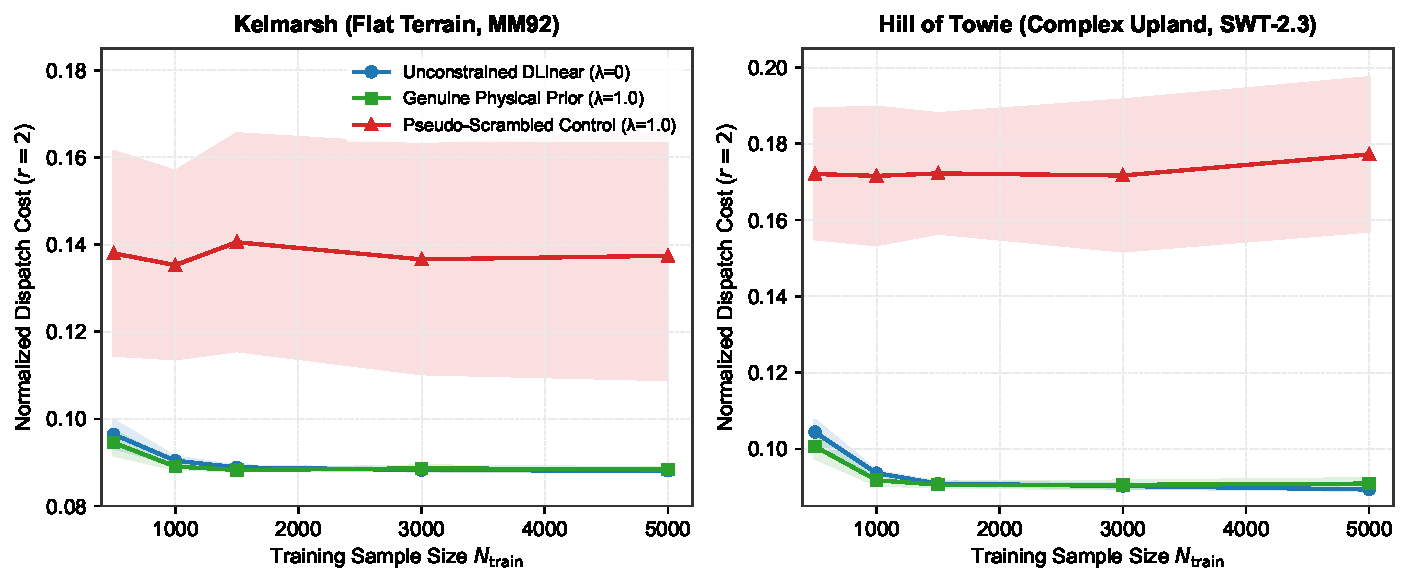
\includegraphics[width=\textwidth]{fig_within_site_learning_curve.pdf}
\caption{Within-Site Learning Curves across Discrete Sample Sizes $N_{\text{train}} \in \{500, 1000, 1500, 3000, 5000\}$ on Kelmarsh and Hill of Towie (Multi-seed means and standard deviations). Holding site topography and turbine hardware constant, authentic empirical priors yield lower dispatch costs in the tested sample-restricted regimes ($N_{\text{train}} \in \{500, 1{,}000\}$, $-2.00\%$ on Kelmarsh and $-3.62\%$ on Hill of Towie at $N=500$). As training volume expands, this advantage attenuates; at the largest evaluated training budget ($N_{\text{train}} = 5{,}000$), unconstrained data-driven models close the gap and slightly reverse the ranking (+0.33\% on Kelmarsh, +1.73\% on Hill of Towie). In contrast, form-matched scrambled priors under strong regularization ($\lambda=1.0$) induce severe dispatch cost penalties ($+43\%$ to $+98\%$) across all evaluated sample regimes.}
\label{fig:within_site_learning_curve}
\end{figure*}

In the tested sample-restricted regimes ($N_{\text{train}} = 500$ and $N_{\text{train}} = 1{,}000$), embedding the authentic empirical power curve prior ($\lambda=1.0$) provides clear downside risk protection:
\begin{itemize}[leftmargin=*]
\item At $N_{\text{train}} = 500$, normalized dispatch cost decreases from $0.09648 \pm 0.00314$ to $0.09455 \pm 0.00285$ ($-2.00\%$) on Kelmarsh, and from $0.10444 \pm 0.00312$ to $0.10066 \pm 0.00307$ ($-3.62\%$) on Hill of Towie.
\item At $N_{\text{train}} = 1{,}000$, the genuine prior maintains an advantage on both sites ($0.09241$ vs.\ $0.09365$, $-1.32\%$ on Kelmarsh; $0.09681$ vs.\ $0.09902$, $-2.23\%$ on Hill of Towie).
\end{itemize}

However, as training volume increases across the intermediate budgets ($N_{\text{train}} = 1{,}500$ and $3{,}000$), the margin of advantage steadily attenuates. At the largest evaluated training budget ($N_{\text{train}} = 5{,}000$), unconstrained DLinear achieves a dispatch cost of $0.08812 \pm 0.00022$ on Kelmarsh and $0.08936 \pm 0.00023$ on Hill of Towie, closing the gap and slightly outperforming the fixed genuine prior ($0.08841 \pm 0.00039$, $+0.33\%$ on Kelmarsh; $0.09091 \pm 0.00131$, $+1.73\%$ on Hill of Towie). Throughout all evaluated sample sizes, form-matched scrambled negative controls inflict severe performance degradations ($+43\%$ to $+98\%$), confirming that unaligned priors remain destructive regardless of sample availability.

\paragraph{Conceptual Interpretation}
The observed learning curves are consistent with a conceptual hypothesis in which the regularizing value of variance reduction diminishes as sample availability increases, while structural approximation bias becomes increasingly consequential. Under this interpretive perspective, in sample-restricted windows, unconstrained models are hypothesized to be vulnerable to elevated estimation variance that an empirical power curve helps suppress by constraining the hypothesis space. Conversely, purely data-driven representations can fit the observed input--output relationship more flexibly as training coverage expands; under these well-sampled conditions, a rigid, static prior can act as a structural approximation bias that constrains the model from fitting nuanced aerodynamic interactions. We emphasize that this bias--variance trade-off is a conceptual interpretation consistent with---not formally identified or proven by---the empirical learning curves, as scalar bias and variance components were not directly decomposed or measured from empirical data.

\paragraph{Joint Operating Envelope}
Taken together, the learning-curve experiments (at $\lambda=1.0$) and separate penalty-sensitivity evaluations suggest that both data availability and regularization strength govern the operating envelope. In the absence of a dense factorial grid across multiple $N \times \text{multiple } \lambda$ values, we characterize this dependency as a joint empirical tendency rather than a statistically proven interaction.

\subsection{Continuous Prior Corruption and Engineering Drift}
To test whether prior vulnerability is restricted to total permutation, we evaluated continuous prior perturbation and engineering drift models on Penmanshiel (Figure~\ref{fig:corruption_gradient}).

\begin{figure*}[!t]
\centering
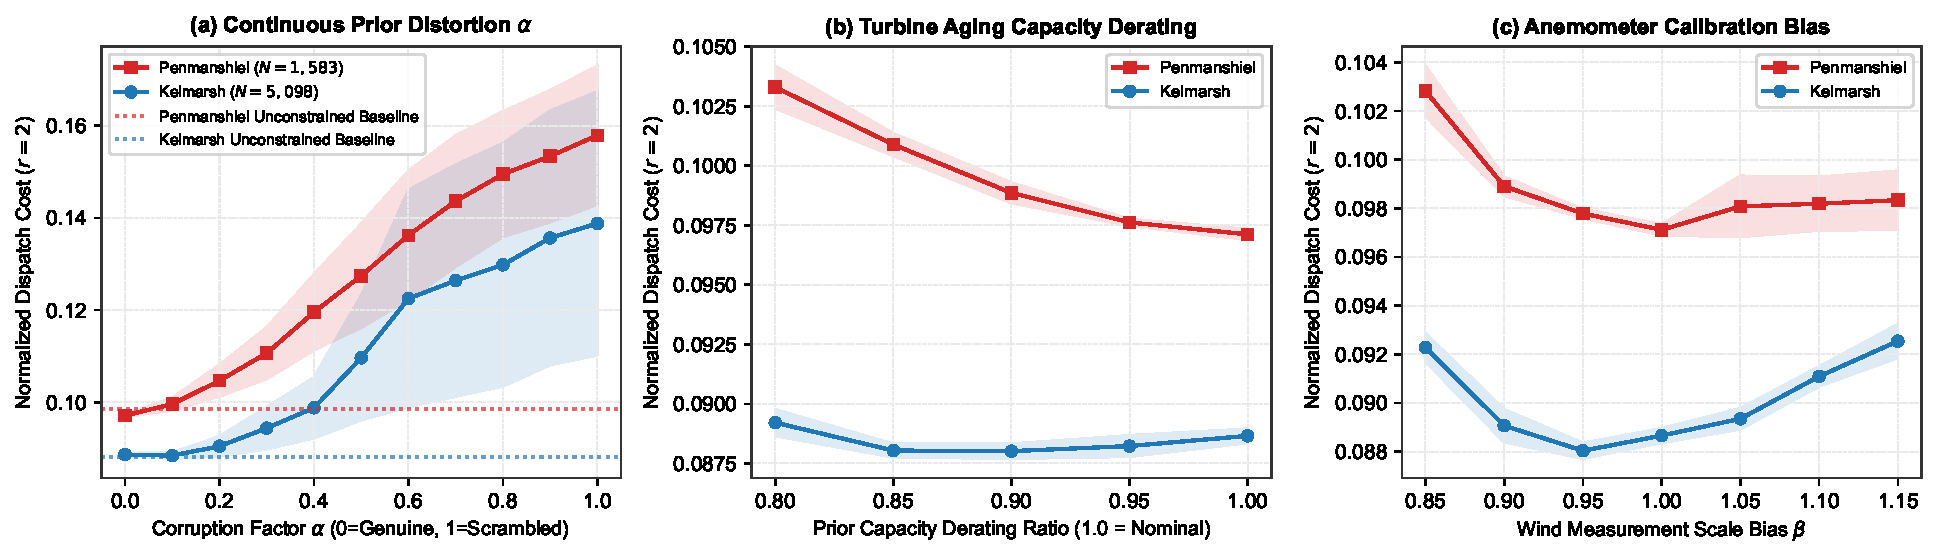
\includegraphics[width=\textwidth]{fig_prior_corruption_gradient.pdf}
\caption{Continuous Prior Corruption and Engineering Drift Severity Response Curves. (a) Continuous interpolation between authentic and scrambled priors $\alpha \in [0.0, 1.0]$: on Penmanshiel, the tested corruption trajectory crosses the unconstrained baseline around an empirical crossover region of $\alpha \approx 0.07$. (b) Turbine aerodynamic aging: capacity derating exceeding 10\% flips nominal physical priors into economic penalties under the evaluated configuration. (c) Anemometer sensor calibration drift: Penmanshiel retains an advantage under positive wind speed drift up to $+15\%$, whereas negative sensor under-reporting systematically inflates shortfall.}
\label{fig:corruption_gradient}
\end{figure*}

\paragraph{Continuous Corruption Interpolation (\texorpdfstring{$\alpha \in [0.0, 1.0]$}{alpha in [0.0, 1.0]})}
We constructed a continuous perturbation trajectory parameterized by $\alpha \in [0.0, 1.0]$, linearly blending the authentic power curve with its scrambled permutation. As shown in Figure~\ref{fig:corruption_gradient}a, dispatch cost degrades monotonically with perturbation severity. On Penmanshiel, the tested corruption trajectory crosses the unconstrained baseline around an empirical crossover region of $\alpha \approx 0.07$: costs rise from $0.09712 \pm 0.00031$ at $\alpha = 0.0$ to $0.09958 \pm 0.00042$ at $\alpha = 0.1$. At $\alpha = 0.2$, normalized dispatch cost reaches $0.10469 \pm 0.00338$ (a $+5.9\%$ degradation relative to unconstrained models). We emphasize that these values are empirical crossover locations along the evaluated perturbation grid, not population-level physical thresholds, indicating that even modest distortion (under 10\% permutation blend) is sufficient to erode inductive benefits in this configuration.

\paragraph{Turbine Aerodynamic Aging and Derating}
In operational wind fleets, blade erosion, leading-edge roughness, and mechanical aging cause progressive aerodynamic derating. In the evaluated Penmanshiel configuration, simulating turbine capacity derating reveals that derating exceeding 10\% flips nominal physical priors into net economic penalties (Figure~\ref{fig:corruption_gradient}b), as the network regularizes against an un-derated historical envelope that exceeds the turbine's degraded capability. This 10\% threshold reflects the evaluated operating margin where representation bias overtakes variance reduction.

\paragraph{Anemometer Calibration Drift}
Simulating anemometer measurement drift ($\pm 15\%$) reveals asymmetric operational tolerances (Figure~\ref{fig:corruption_gradient}c). On Penmanshiel, the model retains a modest advantage over unconstrained baselines under positive wind speed drift up to $+15\%$ ($0.09833$ vs.\ $0.09852$). In contrast, negative wind speed under-reporting systematically depresses predicted power, triggering substantial shortfall penalties during high-wind ramp events.

\subsection{Sensitivity to Training-Loss Proxy Staleness}
Many physical constraint formulations rely on meteorological proxies (such as supervisory anemometer readings) to query empirical power curves during loss evaluation. To assess sensitivity to proxy latency in the absence of forward numerical weather predictions, we performed a parametric lag scan across $k \in \{6, 12, 18, 36\}$ steps (representing 1\,h to 6\,h delay in the training proxy; Figure~\ref{fig:ablation_3d}c).

In the Hill of Towie lag scan, decision risk exceeds the unconstrained reference ($0.08913$) by the first evaluated lag $k=6$ (1\,h delay, normalized dispatch cost $0.09011 \pm 0.00008$) and deteriorates monotonically through $k=36$ ($0.09246 \pm 0.00006$). On Kelmarsh, dispatch cost rises from $0.08867$ ($k=6$) to $0.09034$ ($k=36$). On Penmanshiel, dispatch cost escalates from $0.09996$ ($k=6$) to $0.10425$ ($k=36$). Because $k=6$ is the minimum non-zero lag evaluated in this discrete grid, this observation establishes that latency begins degrading operational value within the first hour of proxy delay, while more granular sub-hour transitions remain unobserved.

This experiment isolates the sensitivity of offline training objectives to temporal misalignment between the forecast horizon and the historical weather proxy used to index the power curve. It demonstrates that when contemporaneous or forward meteorological forecasts are unavailable, regularizing predictions against stale weather proxies monotonically degrades downstream dispatch performance.

\subsection{Cross-Backbone Architectural Sensitivity Probe (PatchTST)}
To examine whether boundary behaviors are specific to linear decomposition architectures, we evaluated PatchTST \cite{nie2023patchtst} across 60 independently trained models (3 farms $\times$ 4 constraint conditions $\times$ 5 random seeds; Table~\ref{tab:patchtst_and_rules}) under nominal regularization ($\lambda=0.01$).

\begin{table*}[!t]
\centering
\footnotesize
\renewcommand{\arraystretch}{0.85}
\setlength{\tabcolsep}{2.8pt}
\caption{Exploratory Cross-Backbone Architectural Sensitivity Analysis: Modern Deep Transformer (PatchTST, ICLR 2023) under BSC 30-Minute Physical Netting Settlement (5-Seed Mean $\pm$ Std).}
\label{tab:patchtst_and_rules}
\begin{threeparttable}
\begin{tabularx}{\textwidth}{p{2.0cm}p{3.0cm}l>{\centering\arraybackslash}X>{\centering\arraybackslash}X>{\centering\arraybackslash}X>{\centering\arraybackslash}X}
\toprule
\textbf{Site} & \textbf{PatchTST Model} & \textbf{Policy} & \textbf{RMSE} & \textbf{Normalized Dynamic} & \textbf{Shortfall Cashout} & \textbf{Balancing Imbalance} \\
 & \textbf{Variant} & & \textbf{(pu)} & \textbf{Cost $\text{Cost}_{\text{dyn}}$} & \textbf{(\pounds/(turb$\cdot$yr))} & \textbf{Cashflow (\pounds/(turb$\cdot$yr))} \\
\midrule
\multirow{6}{=}{\textbf{Hill of Towie}\\(48.3 MW, Upland)} & \multirow{2}{=}{Unconstrained PatchTST} & Uncalibrated & 0.1176 & 0.10518 & \pounds 21,753.77 & \pounds 12,292.64 \\
 &  & \textbf{Calibrated} & 0.1202 & 0.10220 & \pounds 18,168.11 & \pounds 20,822.29 \\
 & Power Curve ($\lambda=0.01$) & Calibrated & 0.1201 & 0.10212 & \pounds 18,163.56 & \pounds 20,765.01 \\
 & \multirow{2}{=}{Distribution Prior ($\lambda=0.01$)} & Uncalibrated & 0.1162 & 0.10507 & \pounds 22,362.12 & \pounds 9,762.57 \\
 &  & \textbf{Calibrated} & 0.1192 & 0.10129 & \textbf{\pounds 17,935.67} & \textbf{\pounds 20,253.61} \\
\cmidrule(lr){1-7}
\multirow{6}{=}{\textbf{Kelmarsh}\\(12.3 MW, Flat)} & \multirow{2}{=}{Unconstrained PatchTST} & Uncalibrated & 0.1092 & 0.10889 & \pounds 22,630.77 & \pounds 4,523.36 \\
 &  & \textbf{Calibrated} & 0.1118 & 0.10222 & \textbf{\pounds 16,808.90} & \textbf{\pounds 17,411.89} \\
 & Power Curve ($\lambda=0.01$) & Calibrated & 0.1117 & 0.10212 & \pounds 16,774.31 & \pounds 17,431.54 \\
 & \multirow{2}{=}{Distribution Prior ($\lambda=0.01$)} & Uncalibrated & 0.1075 & 0.10870 & \pounds 23,336.46 & \pounds 1,528.06 \\
 &  & \textbf{Calibrated} & 0.1097 & 0.10075 & \pounds 16,681.41 & \pounds 16,046.77 \\
\cmidrule(lr){1-7}
\multirow{6}{=}{\textbf{Penmanshiel}\\(28.7 MW, Upland)} & \multirow{2}{=}{Unconstrained PatchTST} & Uncalibrated & 0.1268 & 0.12107 & \pounds 26,956.48 & \pounds 3,001.45 \\
 &  & \textbf{Calibrated} & 0.1304 & 0.11270 & \pounds 19,129.15 & \pounds 20,453.24 \\
 & Power Curve ($\lambda=0.01$) & Calibrated & 0.1303 & 0.11264 & \pounds 19,118.38 & \pounds 20,444.41 \\
 & \multirow{2}{=}{Distribution Prior ($\lambda=0.01$)} & Uncalibrated & 0.1265 & 0.11729 & \pounds 24,606.87 & \pounds 6,473.07 \\
 &  & \textbf{Calibrated} & 0.1300 & 0.11134 & \textbf{\pounds 18,338.64} & \textbf{\pounds 21,117.53} \\
\bottomrule
\end{tabularx}
\begin{tablenotes}[flushleft]
\footnotesize
\item \textbf{Notes}: Exploratory sensitivity results for PatchTST (ICLR 2023, patch length 6, stride 4, channel-independent RevIN) evaluate capacity-aligned architectural sensitivity under identical BSC 30-minute physical netting settlement. Results confirm site-dependent divergence: at flat, high-SNR Kelmarsh, unconstrained PatchTST secures higher balancing cashflow (+\pounds 1,365.12/(turb$\cdot$yr) over distribution prior); at upland Penmanshiel and Hill of Towie, distribution regularization provides inductive protection, saving \pounds 790.51/(turb$\cdot$yr) and \pounds 232.44/(turb$\cdot$yr) in single-sided shortfall. Evaluated under univariate power input and fixed $\lambda=0.01$ as an architectural sensitivity probe without hyperparameter retuning.
\end{tablenotes}
\end{threeparttable}
\end{table*}

As detailed in Table~\ref{tab:patchtst_and_rules}, PatchTST confirms that distribution priors consistently reduce dynamic shortfall expenditure across all three wind farms (saving \pounds 232.44, \pounds 127.49, and \pounds 790.51/(turb$\cdot$yr) on Hill of Towie, Kelmarsh, and Penmanshiel, respectively), indicating that defensive shortfall reduction is preserved in non-linear patch representations. However, net balancing cashflow exhibits a sharp architectural divergence: on Hill of Towie, distribution regularization decreases net cashflow by \pounds 568.68/(turb$\cdot$yr) under PatchTST, inverting the positive cashflow increment observed under DLinear.

Furthermore, on Penmanshiel in the sample-restricted regime, simple empirical baselines (Ridge regression at $0.09744$ and Persistence at $0.09586$) outperform all constrained deep networks (PatchTST at $0.11134$). This confirms that external physical loss penalties cannot uniformly compensate for deep parameter overfitting when training data is severely restricted.
